\section{Introduction}
\label{sec:introduction}

As frontier AI systems are pretrained on web-scale data, test set contamination has become a critical concern for accurately assessing their capabilities \citep{sainz2023nlp,schaeffer2023pretrainingtestsetneed,xu2024benchmarkdatacontaminationlarge,deng2024unveiling,reuel2025open}. 
Evaluation aims to measure generalization on tasks the model has never seen, yet the sheer scale of modern pretraining makes such contamination increasingly likely \citep{brown2020language, du2022glam, wei2022finetuned,chowdhery2022palmscalinglanguagemodeling,touvron2023llama2openfoundation}. 

Prior research has sought to quantify the impact of test set contamination, also known as leakage, through two primary lenses. \textit{Statistical approaches} attempt to detect contamination or estimate its influence by modifying the test set, for example, by reordering, rephrasing, or replicating benchmark problems, e.g., \citep{oren2023proving, ni2025trainingbenchmarkneed, shi2024detecting, golchin2023data,golchin2024time,roberts2024to, wang2025generalization, zhang2024carefulexaminationlargelanguage}.
In comparison, \textit{controlled approaches} -- which offer the most rigorous measurement -- intentionally contaminate pretraining corpora to quantify how specific dosages of leakage inflate performance, e.g., \citep{magar2022data,jiang2024investigatingdatacontaminationpretraining,oren2023proving,yao2024data, wang2025generalization,kocyigit2025overestimation,bordt2025howmuch}.
For a more thorough discussion, please see Appendix~\ref{app:sec:related_work} Related Work.

\begin{figure*}[t!]
\centering
\hspace{-1em}
\begin{minipage}[t]{0.47\textwidth}
    \vspace{0pt}
    \centering
    % \includegraphics[width=\linewidth]{figures/01_revised_figures/pretraining_schematic.png}
    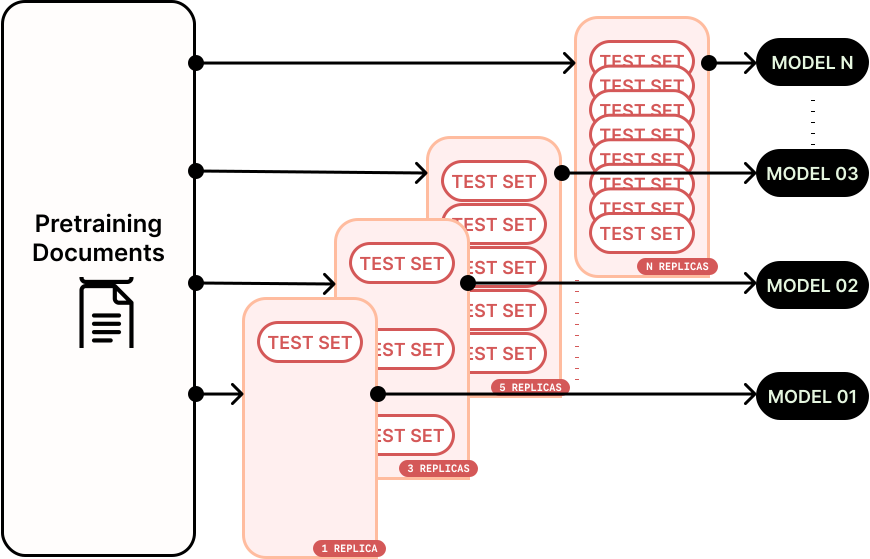
\includegraphics[width=\linewidth]{figures/schematic.pdf}
\end{minipage}%
\hspace{0.1em}
\begin{minipage}[t]{0.49\textwidth}
    \vspace{0pt}
    \centering
    \includegraphics[width=\linewidth]{figures/11_math_qwen3_pt_math_verify/y=math_verify_by_num_parameters_by_num_replicas.pdf}    
    % \includegraphics[width=\linewidth]{figures/10_math_qwen3_pt_cross_entropy/y=loss_by_num_parameters_by_num_replicas.pdf}
    \includegraphics[width=\linewidth]{figures/10_math_qwen3_pt_cross_entropy/y=loss_ratio_by_num_parameters_by_num_replicas.pdf}
\end{minipage}
    \caption{\textbf{Performance on Generative Benchmarks Increases with Test Set Contamination and Model Size.} \text{Schematic:} We pretrained compute-optimal language models ($34$M--$344$M parameters) on corpora containing different replicas of the MATH test set ($0$--$3162$). Evaluation used greedy decoding (temperature $=0$). \textbf{Left:} As contamination (quantified by the number of test set replicas in the pretraining corpus) increases, Math Verify scores (top) rise and cross entropies on the test set (bottom) fall, consistent with discriminative evaluations, with a sharp improvement around $100$. \textbf{Right:} The ratio in the loss on the MATH test set between $R$ replicas and $0$ replicas grows with model size, meaning larger models benefit more from test set contamination for the same number of replicas (consistent with prior findings that larger models memorize more readily \citep{tirumala2022memorization, carlini2023quantifying, biderman2023emergent}; see Appendix~\ref{app:sec:related_work}).}
    \label{fig:math_verify_ce_temp_0}
\end{figure*}

While foundational, these investigations have predominantly focused on \textit{discriminative} benchmarks like classification or multiple-choice question-answering (MCQA). For example, \citet{magar2022data} used SST-2 \citep{socher2013sst} (classification). \citet{jiang2024investigatingdatacontaminationpretraining} used SST-2 (classification), MMLU \citep{hendrycks2021measuring} (MCQA), SQuAD \citep{rajpurkar2016squad} (MCQA), and CNN/Daily Mail (fill-in-the-middle) \citep{nallapati2016abstractive}. \citet{oren2023proving} used 7 MCQA benchmarks and 1 mathematical problem solving benchmark (GSM8K) \citep{cobbe2021trainingverifierssolvemath}, \citet{yao2024data} used 3 MCQA benchmarks while \citet{bordt2025howmuch} used 7 MCQA benchmarks.

However, with the rapid advancement of model capabilities and the advent of reasoning models \citep{openai2024openaio1card,comanici2025gemini25pushingfrontier,xu2025largereasoningmodelssurvey}, the field is shifting towards benchmarks for which the model must generate an answer rather than choose between provided answers.
Whether test set contamination has the same effect on generative evaluation as on discriminative evaluations is unclear.
Discriminative evaluations typically require the model to place higher probability mass on the correct choice than on a small number of alternative incorrect choices \citep{gao2024evalharness, schaeffer2025elusive}, and candidate choices are often only a couple of tokens long.
In contrast, generative evaluations require the model to produce solutions spanning tens-to-thousands of tokens without straying from the memorized path, and introduce new considerations such as the sampling temperature \citep{ackley1985learning}, the sampling algorithm (e.g., top-k \citep{fan2018topk}, top-p \citep{holtzman2020topp}) and the solution length.


\begin{figure*}[t!]
    \centering
    \includegraphics[width=0.9\linewidth]{figures/20_gen_eval_contamination_vs_compute/y=loss_x=flop_hue=num_replicas.pdf}
    \includegraphics[width=0.9\linewidth]{figures/20_gen_eval_contamination_vs_compute/y=fit-params_x=num-replicas_col=param_setting=full-fits.pdf}
    \caption{\textbf{Scaling Laws Suggest Including A Single Test Set Replica Achieves Lower Loss Than the Irreducible Error of the Uncontaminated Corpus.} \textbf{Top:} For each scaling series pretrained on corpora contaminated with $R$ replicas of the MATH test set, we fit scaling laws $\mathcal{L}(C, R) = E(R) + C_0(R) \cdot C^{-\alpha(R)}$, where $C=6\, N \, D$ is the pretraining compute. 
    Almost all contaminated models achieve lower cross entropy on the MATH test set than the irreducible error of training on uncontaminated data (horizontal purple line).
    \textbf{Bottom:} Increasing test set contamination reduces the irreducible error $E(R)$ from $3.594$ at $R=0$ to $0.0347$ at $R=316$. Larger values of $R$ also increase the compute prefactor and compute exponent.
    The functional form achieves average fitting error $< 10^{-2}$ for all $R$.
    }
    \label{fig:contamination_scaling_laws}
\end{figure*}

In this work, we quantitatively study the effects of test set contamination on generative evaluations, focusing on the widely used MATH benchmark \citep{hendrycks2021measuringmathematicalproblemsolving}. 
We pretrain dozens of language models on corpora contaminated with varying numbers of test set replicas, sweeping across model sizes, sampling temperatures, and token budgets. 
% Our findings reveal that while generative contamination shares some similarities with discriminative settings, it introduces new interactions between memorization and generalization.
We make the following contributions:
%
\begin{itemize}
    \item \textbf{Pretraining (Scaling \& Irreducible Error):} We quantify how contamination impacts pretrained models. We find that performance increases with the number of test set replicas in the pretraining corpus and with model size, similar to discriminative settings. Under standard scaling law assumptions, we discover that including even a single replica of the test set enables models to achieve a lower loss than the estimated irreducible error of the uncontaminated corpus.
    
    \item \textbf{Further Training (Overtraining \& Supervised Finetuning):} We find that training beyond compute-optimal with fresh data dilutes increased performance from contamination, similar to discriminative settings. We then show that SFT on the training data has opposing effects, depending on the amount of contamination in pretraining: performance improves for low contamination, but worsens for high contamination.

    \item \textbf{Inference (Temperature \& Solution Length):} We identify distinct factors that modulate memorization during generation: increasing sampling temperature and increasing solution sequence length each reduce model performance, as models struggle to regurgitate long sequences without decohering.

    \item \textbf{Correction to Evaluation Library:} We identify and fix a critical implementation error in the widely used EleutherAI LM Evaluation Harness \citep{gao2024evalharness} for Math Verify Scores. Our correction ensures that valid reference solutions are accurately scored as correct (raising gold reference solutions' scores from $\mathord{\sim}$70\% to 100\%), a necessary step for trustworthy reporting on mathematical benchmarks.
\end{itemize}
